\documentclass[a4paper, 11pt]{article}
\setlength{\topmargin}{-0.5in}
\setlength{\textheight}{9.5in}
\setlength{\oddsidemargin}{-.1in}
\setlength{\textwidth}{6.5in}
\setlength{\parskip}{1em}
\usepackage{graphicx}
\graphicspath{ {images/} }
\usepackage{datetime}

\newdateformat{monthyeardate}{%
  \monthname[\THEMONTH], \THEYEAR}

\date{}
\begin{document} 

\LARGE\title{Real Time Tempo Analysis of Drum Beats}

\LARGE\author{Author: \textbf{Philip Hannant}, Supervisor: \textbf{Professor Steve Maybank}\\
\\Birkbeck, University of London\\
Department of Computer Science and Information Systems\\
\\Project Report\\
MSc Computer Science\\
\\\monthyeardate\today
}





\normalsize


\maketitle
\newpage
\tableofcontents
\clearpage

\section*{Abbreviations}
\begin{tabular}{l p{4.5in}  }\\
\textbf{BPM} & Beats Per Minute\\
\textbf{DWT} & Discrete Wavelet Transform\\
\textbf{FT} & Fourier Transform\\
\textbf{JSON} & Javacript Object Notification\\
\textbf{IDE} & Integrated Development Environment\\
\textbf{STFT} & Short-Time Fourier Transform\\
\textbf{TDD} & Test Driven Development\\
\end{tabular}

\section*{Definitions}
\begin{tabular}{l p{4.5in}  }\\
\textbf{Acoustic Drum Kit} & A collection of drums and cymbals which do not have electronic amplification. Typically made up of a bass drum, snare drum, tom-toms, hi-hat and 1 or more cymbals.\\\\
\textbf{Beat} & For the purpose of this project a beat will be defined as the sequence of equally spaced pulses used to calculate the tempo being played by the drummer.\\\\
\textbf{Downbeat} & Refers to beat one of a measure of music, called a downbeat to correspond to the motion a conductor's arm [1].\\\\
\textbf{Drum Module} & The device which serves as a central processing unit for an electronic drum kit, responsible for producing the sounds of the drum kit.\\\\
\textbf{Electronic Drum Kit} & An electrical device which is played like an acoustic drum kit, producing sounds from a stored library of instruments and samples.\\\\
\textbf{Measure/Bar} & A measure or bar is a segment of time made up by a predetermined number of beats, for example a piece of music with a 4/4 time signature will have 4 beats in every measure/bar [2].\\\\
\textbf{MIDI} & Musical Instrument Digital Interface is a protocol developed in the 1980's to allow electronic instruments and other digital musical tools to communicate with each other [3].\\\\
\end{tabular}
\clearpage

\maketitle{} \section{Introduction}

This project report presents my aim to develop a real-time drum beat tempo analysis system using different beat detection algorithms which is able to record the perfomance of each method concurrently when an extensive set of drum samples, representing a real drummer's perfomance, is processed through the system.

\maketitle{} \subsection{Drumming Training Tools Background}
Timing is the fundamental skill any good drummer should possess and is the staple by which they will be judged. For many years the only training tool available to a drummer to improve their timing was the metronome. An instrument used to mark musical tempo, erroenously attributed to Johann Nepomuk Maelzel in 1815 but was actually invented by a Dutchman, Dietrich Nikolaus Winkel a year earlier. The traditional metronome, based on Winkel's original design is a hand-wound clockwork instrument that uses a pendulum swung on a pivot to generate the ticking which depicts the desired tempo \cite{brit-metro} is still used today by musicians. \par


For drummers however the electronic versions of the metronome are much more widely used, to the point that metronomes are now developed with functionality specifically tailored to a drummers training requirements. The Tama Rhytham Watch was the first metronome designed specifically for drummers, providing enough volume to be used with real drums as well as allowing for the use of different time signatures and preset set rhythm patterns to help improve perfomance. (Tama rhythm watch image) \par

Following the development of MIDI driven electronic drum kit came the development of more advanced training tools that now were able to provide live feedback to drummer during any given perfomance. Today the leaders in this field are Roland, their v-drums line provide a variety of tutition packages including the SCOPE and more recently the COACH system provided in the v-drum modules, the v-drum Rhymthm Coach line is an advanced version of the traditional drummers practice pad and the extensive DT-1 V-Drums tutor software package. Roland have even now gamified this field with their latest release, the V-Drums Friend Jam app. The application itself provides the player with live feedback and evaluates each performance in order to provide the player with a score which they can share over social media. \par

The aim of this project is to investigate whether some of the current beat detection algorithms available would be accurate enough to provide the basis for a training tool for dummers using an acoustic drum kit as opposed to an electronic drum kit. \par

\maketitle{} \subsection{Drum Musical Theory}
In order to understand the fundamentals of musical timing some theory needs to be examined but beforehand the concept of a drummer's time must be considered. Time, in a drumming sense is an informal term used to describe the consistent rhythmic pattern that a drummer will play on the hi-hat or ride cymbal \cite{drum-bible} and it can be considered one of the most important components of any drum beat. 

\maketitle{} \subsubsection{Notation}
Drum music notation is written on staff that is made up of five individual lines, the clef is found on the far left of the staff which indicates the pitch of the notes \cite{oxford-comp} and as percussion instruments are non-pitched they use the percussion-clef. On traditional musical notation the lines and spaces between represent a tonal where as for drum notation, notes written on lines or spaces indicate a certain drum or cymbal. The staff is seperated into individual measures which are known as bars \cite{drum-note} and it is these bars that are the basis of musical time. 

\maketitle{} \subsubsection{Time Signatures}
Time signatures appear on the staff just after the clef and are written as a fraction where the top number indicates the number of beats that there are in a bar. With the bottom number representing the size of the note that makes up the duration of one beat. For example the straight time four four (4/4) or common time signature indicates four beats in each bar or measure where each beat is made up of one quarter note \cite{drum-note}. Within these bar lines beats can be further divided by using a technique known as subdivision, which is a method for reducing the pulse or rhythm pattern into smaller parts than those originally written, for example counting a four four (4/4) measure in eighth (1/8) or sixteeth (1/16) notes. 

\maketitle{} \subsubsection{Notes}
The notes used to represent the percussive instrument to be played also provide the duration it should be played for. Notes come in different lengths and the key values are the whole (1/1), half (1/2), quarter (1/4), eighth (1/8) and sixteeth (1/16). For example two eighth notes represent the same time value as a single quarter note. It is possible to divide a note values by three instead of two, these notes are known as triplets. An eighth note triplet is played fifty percent faster than a normal eighth note, therefore for every two eighth notes there will be three eighth note triplets \cite{drum-note}. An example of the eighth-note triplets being used is in a twelve eight (12/8) jazz shuffle, the time element played on the ride cymbal or hi-hat is charaterised by playing the first and third triplet of an eighth-note triplet grouping \cite{drum-bible}.

\maketitle{} \subsubsection{Playing Basics}
With the basics of drum theory covered it is now possible to discuss the key elements of a drum beat, typically for a straight four four (4/4) bar the bass drum will be played on the first and third beat and the snare drum will be played on the second and forth beat both as quarter notes. This is more commonly known as a back beat \cite{drum-bible}. This just leaves the time element which will usually be played on the ride cymbal or hi-hat, this too could be played using quarter notes on the first, second, third and forth beats. However, in order to make the drum pattern more dynamic the time element will usually be played using subdivisions, typically using eighth note subdivisions. The ride cymbal or hi-hat will therefore be played on the first, second, third and forth beats as well as the eighth notes inbetween each quarter note. This can be demostrasted by counting the one-and-two-and-three-and-four-and, where the and represents the subdivided eighth note. Additonally to this technique a drummer will usually ensure that there is difference in the volume of the eighth notes being played on the quarter notes and those being played on the and. This technique of emphasising certain beats is known as accenting. 


\subsection{Beat Detection Background}
Most of the early work on beat detection was as a by-product of research directed at other areas of music. The earliest work in this field can be attributed to H. C. Longuet-Higgins, who in 1976 while researching the psychological theory of how Western musicians perceive rhythmic and tonal relationships between notes. Produced an algorithm that was able to follow the beat of a performance and adjust the perceived tempo accordingly based on whether a note started earlier or later than expected \cite{allen-danneburg}. Longuet-Higgins' work was built on the premise that in order to percieve the rhythmic structure of a melody it is first necessary to identify the time at which each beat occurs \cite{longeut1}, otherwise know as onset detection.\par 

The majority of beat detection methods currently available utilise onset detection is a. The onset of a note is the instant which marks start of the variation in the frequency of a signal, a visualisation of this can be seen in figure 1(currently). Once detected it can then be used to measure the onset times of sonic events\footnote{A sonic event is a singular feature of a piece music which can be made up of one source or many\cite{sonic}, e.g. the hitting of a drum} within a pieceof music\cite{mirex-onset}.



\begin{figure}[h]
	\centering
	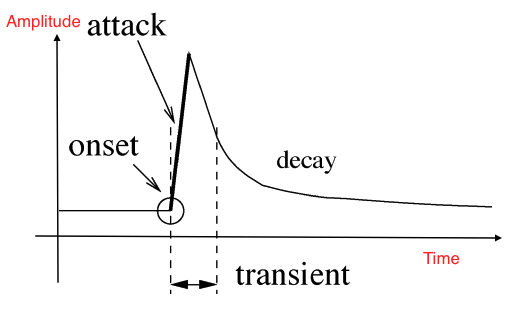
\includegraphics[scale=0.40]{Onset}
	\caption{The onset of a note is the instant which marks start of the variation in the frequency of a signal [11]}
\end{figure}

This process known as onset detection can be considered to be a well-defined task with the simple aim of finding the start time of each musical note \cite{dixon1}.


Since Longuet-Higgins' first work there have been a number of different approaches to beat detection. M. Goto and Y. Muraoka developed a system which learned the frequencies of the bass drum and snare drum, in order to detect events triggered by these instruments during a piece of music [9]. In 2001, Simon Dixon presented Beatroot, an interactive beat tracking and visualisation system which is able to estimate the tempo and times of musical beats in performed music [10]. In the same year Tzanetakis \textit{et al} [11] described an algorithm based on the Discrete Wavelet Transform (DWT) which is capable of detecting the beat attributes of music. 




% Due to the rapidly expanding research being carried out on beat detection, the 1st annual Music Information Retrieval Evaluation eXchange (MIREX) was held in 2005. MIREX includes a contest with the goal of comparing state-of-the-art algorithms for music information retrieval [7]. The topics to be evaluated were proposed by the participants. In the first year, three of the nine topics concerned beat detection (Audio Drum Detection, Audio Onset Detection and Audio Tempo Extraction). 
% There are a number of pieces of software available for real time tempo detection is limited to only a few live bpm detectors available in the App Store\footnote{Apple's application store - itunes.apple.com/uk/appstore‎} and Google Play\footnote{Google's application store for Android devices - play.google.com/store}. An example It is therefore a focus of this project to investigate if the beat detection system Beatroot and Tzanetakis \textit{et al's} [12] method are accurate enough to be implemented in a live tempo drum beat analyser.

\subsubsection{Beatroot}
Beatroot is an audio beat detection system presented by Simon Dixon in 2001 and is described as a ``beat tracking system which finds the times of musical beats and tracks changes in tempo throughout a performance'' [13]. Beatroot works by first processing digital audio data to produce a list of onset (see Figure 2) or event times. The time intervals between these events are then analysed to generate tempo hypotheses concerning the rate and location of beats. Using the tempo hypotheses, searches are carried out to test the different hypotheses about the rate and timing of beats. The results of these searches are ranked and the beat times found in the highest ranked search are returned [10]. 

% \subsubsection{Onset Detection}
% Onset detection is a process used by most of beat detection methods currently available. The onset of a note is the instant which marks start of the variation in the frequency of a signal, a visualisation of this can be seen in figure 2. Once detected it can then be used to measure the onset times of sonic events\footnote{A sonic event is a singular feature of a piece music which can be made up of one source or many[24], e.g. the hitting of a drum} within a pieceof music [9].



\subsubsection{Short-Time Fourier Transform}
To detect the onsets of a piece of digital audio Beatroot uses an onset detection function based on the Short-Time Fourier Transform (STFT). The STFT is a form of Fourier transform (FT) which was developed by Joseph Fourier in 1822 [16], which can be used to find out how much of each frequency exists in a signal. A drawback of the FT is that it is unable to provide any details of when a frequency component occurs in time for non-stationary signals\footnote{Non-stationary signals are signals whose frequency contents changes over time [17].}. A solution to this was to split a non-stationary signal up into a number of smaller segments using a window function, which effectively created a series of stationary\footnote{The frequency contents of a stationary signal does not change over time} signals which the FT could then be applied to. However, this did not fully solve the problem as the size of window function affects the quality of frequency resolution and time resolution:
\begin{itemize}
\item Narrow Window Function $\longrightarrow$  Good Time Resolution, Bad Frequency Resolution
\item Wide Window Function $\longrightarrow$  Bad Time Resolution, Good Frequency Resolution [17]
\end{itemize}

\subsubsection{Discrete Wavelet Transform}
The first literature regarding the wavelet was provided by the mathematician Albert Haar in 1909 [18]. The wavelet transform is a technique for analysing signals which was developed as an alternative to the STFT [11]. Like the STFT, the DWT is able to provide time and frequency information, however, unlike the STFT the DWT is able to do this without the need for a window function. 

\subsubsection{Tzanetakis \textit{et al} Beat Detection Method}
In 2001, Tzanetakis \textit{et al} described how the Discrete Wavelet Transform (DWT) could be used to extract information from non-speech audio [11]. Their beat detection algorithm was based on detecting the most prominent signals which are repeated over a period of time within the analysed audio and was is split into the following steps: 

\begin{enumerate}
\item Signal decomposed into a number of octave frequency bands using the DWT
\item The subsequent time domain information is extracted for each frequency band
\item The data from each band are then summed together and a function to find repeating patterns is applied
\end{enumerate}

As there is no current open source Java implementation of this algorithm. I will attempt to implement a version of this myself, which will be the DWT based beat detection component of this project.









\subsection{Live Audio Processing}
The live audio will be processed using the Javax Sound package. The audio will be captured using a stereo microphone and processed to match CD quality with the Javax Sound AudioFormat class. The Beatroot system was not originally intended to be used as a real time system [19] so currently only works with prerecorded audio. It will therefore be will need to be modified in order for it to work with live audio. 

% \begin{itemize}
% \item Encoding - This will be set to ``PCM.signed'', representing audio encoded to the native linear pulse code modulation, where quantization levels are linearly uniform [15].
% \item Sample Rate - 44,100, set to match CD quality for the number of analog samples which will be analysed per second. 
% \item Sample Size in Bits - 24, based on a sound card with a 24 bit sample depth.
% \item Channels - 2, audio will be captured using a stereo microphone.
% \item Frame Size - 6, where the frame size is the number of bytes in a sample multiplied by the number of channels [17].
% \item Frame Rate - 44,100, same as sample rate.
% \item Big Endian (boolean) - false, as the project will be developed on an Intel core which uses a little-endian architecture\footnote{Endianess refers to the order of bytes which make up a digital word. Big endianess stores the most significant byte at a certain memory address and the remaining bytes being stored in the following higher memory addresses. The little-endian formate reverses the order storing the least significant at the lowest and most significant at the highest memory address [16].}.
% \end{itemize}

\subsection{Implementation of Tzanetakis \textit{et al} Beat Detection Algorithm}
The beat detection algorithm described by Tzanetakis \textit{et al} [11] is based on detecting the most prominent periodicities of a signal and is made up of the following stages:\footnote{A full description of the theory regarding Tzanetakis \textit{et al} beat detection algorithm will be provided in the Project Report.}

\begin{itemize}
\item DWT - First the signal is processed by the DWT into a number of frequency bands 
\item Low Pass Filtering - a low pass filter is then applied to the signal in order to allow the lower frequencies of the signal to be analysed
\item Full Wave Rectification - each frequency band is then converted to one constant polarity (positive or negative)[wiki]. A visual representation can be seen in Figure 4
\item Downsampling - the sampling rate of the signal is decreased by an integer factor [20]
\item Normalisation - each band is then normalised using mean removal
\item AutoCorrelation - an autocorrelation function is then applied to the frequency bands, the first five peaks of this function are detected and their periodicities are calculated in beats per minute
\end{itemize}



If the implementation of this algorithm takes longer than described in the schedule in   section 5. The Matlab implementation created by Eng Eder de Souza [21] will be adapted for use to be used in this system. 




\clearpage



\begin{thebibliography}{99}
\bibitem{brit-metro} 
\textit{https://www.britannica.com/art/metronome}
\bibitem{drum-bible}
Mick Berry and Jason Gianni
\textit{The Drummer's Bible: How to Play Every Drum Style from Afro-Cuban to Zydeco, Second Edition, 2004, See Sharp Press}
\bibitem{oxford-comp}
Alison Latham
\textit{The Oxford Companion to Music, 2002, Oxford University Press}
\bibitem{drum-note}
\textit{http://www.drummagazine.com/lessons/post/drumkey/}
\bibitem{allen-danneburg}
Allen and Dannenberg
\textit{Tracking Musical Beats in Real Time, International Computer Music Conference, International Computer Music Association, 1990, pp. 140-143}
\bibitem{longeut1}
H. C Longuet-Higgins
\textit{Perception of melodies, Nature Vol. 263, 1976, pp. 646-653}
\bibitem{dixon1}
Simon Dixon
\textit{Onset Detection Revisited, Proceedings of the 9th International Conference on Digital Audio Effects, Montreal, September 2006, pp 133-137}
\bibitem{mirex-onset}
\textit{http://www.music-ir.org/mirex/wiki/2016:Audio\_Onset\_Detection}
\bibitem{sonic}
\textit{http://www.ieor.berkeley.edu/~ieor170/sp15/files/Intro-to\_Sonic\_Events\_Campion.pdf}

\end{thebibliography}
\end{document}

